\chapter{Assignment 5}\label{ass5}

\section{Task 1}\label{ass5_t1}

We already switched from jade to indigo for the last assignment, as can be seen in the attached picture from last week.

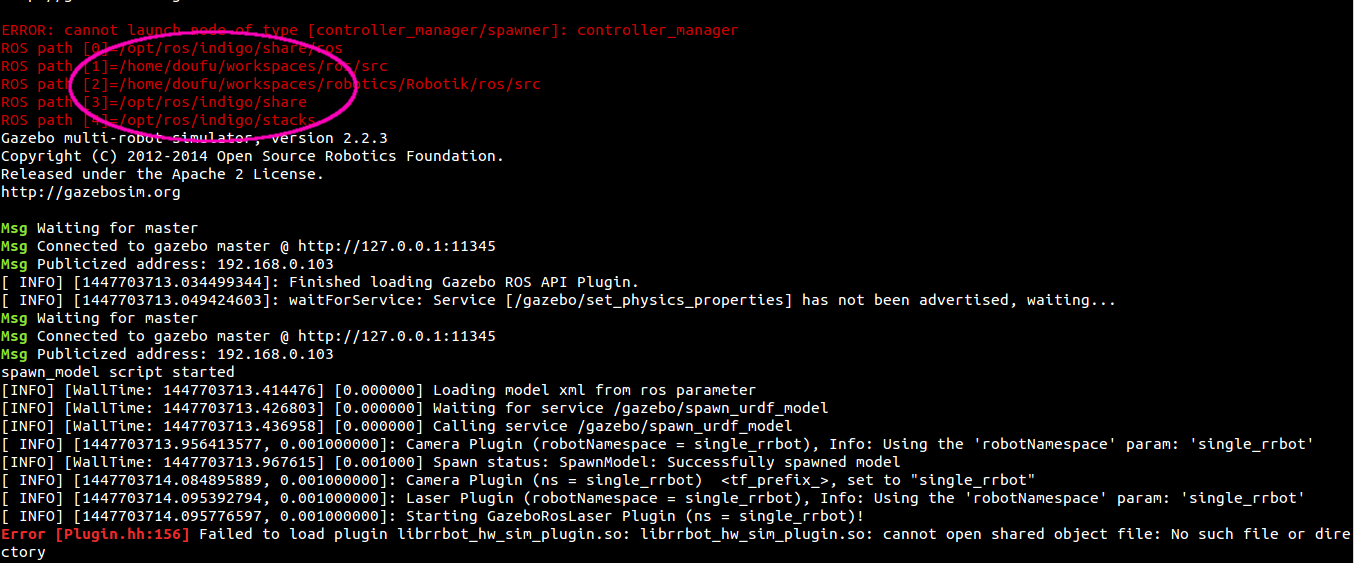
\includegraphics[width=0.75\textwidth]{img/screen_ue5_t1.png}

\section{Task 2}\label{ass5_t2}

Screenshot of the whole car:\\
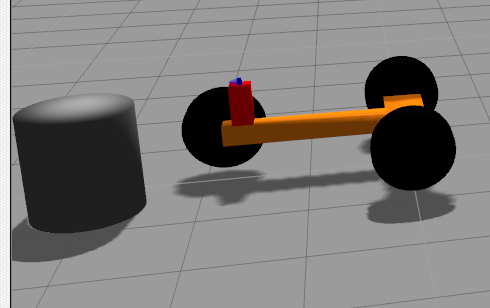
\includegraphics[width=0.75\textwidth]{img/screen_ue5_t2_car.png}\newpage

Screenshot of the camera-picture:\\
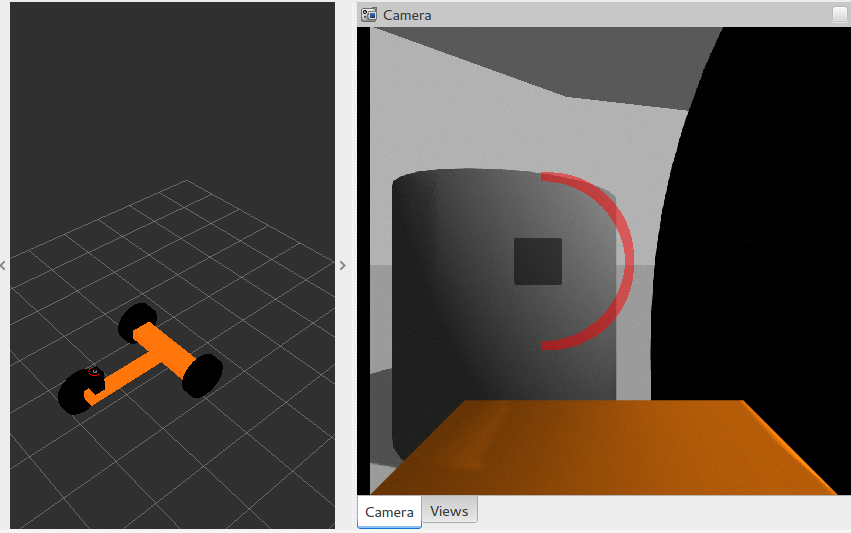
\includegraphics[width=0.75\textwidth]{img/screen_ue5_t2_cam.png}

Screenshot of the point cloud generated by the laser-scanner:\\
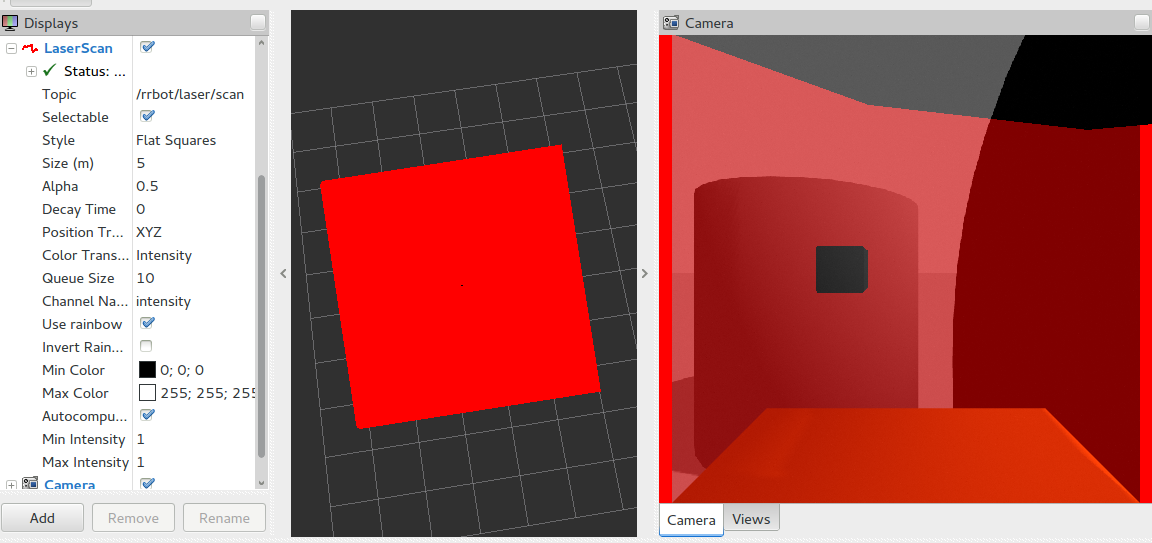
\includegraphics[width=0.75\textwidth]{img/screen_ue5_t2_laser.png}

\section{Task 3}\label{ass5_t3}

\begin{align*}
\alpha_1 &= 0 \\
d_1 &= L_1 \\
\Theta_1 &= 180 \pm \epsilon_{\Theta_1} \\
a_1 &= 0 \\
\\
\alpha_2 &= 90 \pm \epsilon_{\alpha_2} \\
d_2 &= 0 \\
\Theta_2 &= 45 \pm \epsilon_{\Theta_2} \\
a_2 &= 0 \\
\\
\alpha_3 &= 0 \\
d_3 &= 0 \\
\Theta_3 &= 45 \pm \epsilon_{\Theta_3} \\
a_3 &= L_2 \\
\\
\alpha_4 &= 90 \pm \epsilon_{\alpha_4} \\
d_4 &= d_4 \\
\Theta_4 &= 0 \pm \epsilon_{\Theta_4} \\
a_4 &= 0 \\
\\
\Theta_1 &= 180 \pm \epsilon_{\Theta_1} \\
\Theta_2 &= 45 \pm \epsilon_{\Theta_2} \\
\Theta_3 &= 45 \pm \epsilon_{\Theta_3} \\
\end{align*}
Annahme: Der Ursprung von Koordinatensystem 4 ist um $d_4$ vom Ursprung des Koordinatensystems 3 in der Tiefe ($d$) verschoben.
\begin{align*}
T_3^2(\alpha_2,a_2,\Theta_3,d_3) &= \left( \begin{matrix} cos(\Theta_{i}) & -sin(\Theta_i) & 0 & a_{i-1} \\ sin(\Theta_i) \cdot cos(\alpha_{i-1}) & cos(\Theta_i) \cdot cos(\alpha_{i-1}) & -sin(\alpha_{i-1}) & -sin(\alpha_{-1}) \cdot d_i \\ sin(\Theta_i) \cdot cos(\alpha_{i-1}) & cos(\Theta_i) \cdot sin(\alpha_{i-1}) & cos(\alpha_{i-1}) & cos(\alpha_{i-1}) \cdot d_i \\  0 & 0 & 0 & 1\end{matrix} \right) \\
T_3^2(\alpha_2,a_2,45,d_3) &= \left( \begin{matrix} cos(45) & -sin(45) & 0 & 0 \\ sin(45) \cdot cos(45) & cos(45) \cdot cos(45) & -sin(45) & -sin(90) \cdot 0 \\ sin(45) \cdot cos(90) & cos(45) \cdot sin(90) & cos(90) & cos(90) \cdot 0 \\  0 & 0 & 0 & 1\end{matrix} \right) \\
T_3^2(\alpha_2,a_2,45,d_3) &= \left( \begin{matrix} \frac{1}{\sqrt{2}} & -\frac{1}{\sqrt{2}} & 0 & 0 \\ \frac{1}{2} & \frac{1}{2} & -\frac{1}{\sqrt{2}} & 0 \\ 0 & \frac{1}{\sqrt{2}} & 0 & 0 \\  0 & 0 & 0 & 1\end{matrix} \right)
\end{align*}

\section{Task 4}\label{ass5_t4}

\subsection{a)}\label{ass5_t4a}

\begin{align*}
^{0}_3 A(q_1, q_2, q_3) &= ^{0}_1 A(q_1) \cdot ^{1}_2 A(q_2) \cdot ^{2}_3 A(q_3) \\
^{0}_3 A &= \left( \begin{matrix} cos(\Theta_1) & -sin(\Theta_1) & 0 & 0 \\ sin(\Theta_1) & cos(\Theta_1) & 0 & 0 \\ 0 & 0 & 1 & 0 \\ 0 & 0 & 0 & 1\end{matrix} \right) \cdot \left( \begin{matrix} 1 & 0 & 0 & 0 \\ 0 & 1 & 0 & 0 \\ 0 & 0 & 1 & d_2 \\ 0 & 0 & 0 & 1\end{matrix} \right) \cdot \left( \begin{matrix} 1 & 0 & 0 & 0 \\ 0 & 1 & 0 & 0 \\ 0 & 0 & 1 & d_3 \\ 0 & 0 & 0 & 1\end{matrix} \right) \\
^{0}_3 A &= \left( \begin{matrix} cos(\Theta_1) & -sin(\Theta_1) & 0 & 0 \\ sin(\Theta_1) & cos(\Theta_1) & 0 & 0 \\ 0 & 0 & 1 & d_2 \\ 0 & 0 & 0 & 1\end{matrix} \right) \cdot \left( \begin{matrix} 1 & 0 & 0 & 0 \\ 0 & 1 & 0 & 0 \\ 0 & 0 & 1 & d_3 \\ 0 & 0 & 0 & 1\end{matrix} \right) \\
^{0}_3 A &= \left( \begin{matrix} cos(\Theta_1) & -sin(\Theta_1) & 0 & 0 \\ sin(\Theta_1) & cos(\Theta_1) & 0 & 0 \\ 0 & 0 & 1 & d_2 + d_3 \\ 0 & 0 & 0 & 1\end{matrix} \right)
\end{align*}
Beschreibung der Koordinaten des Zielsystems:
\begin{align*}
f &: \mathbb{R}^3 \longrightarrow \mathbb{R}^3 \\
f &= B \\
B &= \left( \begin{matrix} cos(\Theta_1) & -sin(\Theta_1) & 0 \\ sin(\Theta_1) & cos(\Theta_1) & 0 \\ 0 & 0 & d_2 + d_3 \end{matrix} \right) \\
x &= cos(\Theta_1) - sin(\Theta_1) \\
y &= sin(\Theta_1) + cos(\Theta_1) \\
z &= d_2 + d_3
\end{align*}

\subsection{b)}\label{ass5_t4b}

\begin{align*}
\frac{x}{d \Theta_1} &= -sin(\Theta_1) - cos(\Theta_1)\\
\frac{x}{d d_2} &= 0 \\
\frac{x}{d d_3} &= 0 \\
\\
\frac{y}{d \Theta_1} &= -sin(\Theta_1) + cos(\Theta_1) \\
\frac{y}{d d_2} &= 0 \\
\frac{y}{d d_3} &= 0 \\
\\
\frac{z}{d \Theta_1} &= 0 \\
\frac{z}{d d_2} &= 1 \\
\frac{z}{d d_3} &= 1 \\
\end{align*}

\subsection{c)}\label{ass5_t4a}

\begin{align*}
J(q) &= \left( \begin{matrix} -sin(q_1)-cos(q_1) & -sin(q_1)+cos(q_1) & 0 \\ 0 & 0 & 1 \\ 0 & 0 & 1 \end{matrix} \right)
\end{align*}
